\documentclass[22pt]{beamer}
\usepackage[utf8]{inputenc}
\usepackage{algorithm2e}

\usetheme[numbering=progressbar]{focus}
\definecolor{main1}{RGB}{159, 0, 14}
\definecolor{main2}{RGB}{80, 0, 5}
\definecolor{background}{RGB}{242, 236, 236}

\newcommand{\nologo}{\logo{}}
\title{Extension of the computation of density to non-diagonal band occupations with the KGB parallelization}

%\subtitle{Applied to DFT+DMFT}

\author{T.~Cavignac}

\institute{
  CEA DAM Ile-de-France
  \and
  École Centrale de Lyon
}

\date{\textsc{Abinit} developer Workshop, Mai 2019}

\logo{
\includegraphics[height=1.5cm]{pic/logo-cea.png}}

\begin{document}
  \frame{\titlepage}

  \nologo

  \begin{frame}
    \frametitle{Table of Contents}
    \tableofcontents
  \end{frame}

  \section{Non local density, DMFT and DFT}
  \begin{frame}
  \frametitle{The DMFT, a non local density theory}
  The Dynamic Mean Field Theory (DMFT) is one of the theory developed
  to address the problem of correlated electrons in transition metals 
  and lanthanides.\\
  It deals with non-local density and is totally different from the DFT.\\
  To integrate it to \textsc{Abinit}, its output is represented as a non
  diagonal matrix of occupations of the Kohn-Sham vectors from the DFT part of \textsc{Abinit}.\\
  Then the density is computed from the Kohn-Sham vectors and this matrix.
\end{frame}

\begin{frame}
  \frametitle{From DFT density to DMFT+DFT density}
  Density expressed in terms of Kohn-Sham vectors and occupations:
  \begin{equation}
    n(\vec{r}) = \sum_{i \in \text{bands}} d_i~\phi_i(\vec{r})^* \phi_i(\vec{r})
  \end{equation}

  With non-diagonals occupations

  \begin{equation}
    n(\vec{r}) = \sum_{i, i' \in \text{bands}} d_{i,i'}~\phi_{i'}(\vec{r})^* \phi_i(\vec{r})
  \end{equation}
  \alert{We have now to compute products of vectors from different bands}
\end{frame}


  \section{paral\_kgb and the repartition of data}
  \begin{frame}
  \frametitle{Reminder on Abinit parallelization}
  
  The \texttt{paral\_kgb} mode imply:
  \begin{itemize}
    \item Parallelization over $k$ vectors, which is trivial because
    they are always orthogonal.
  \end{itemize}

  And depending on the context one of:

  \begin{itemize}
    \item Parallelization over \emph{plane waves} ($g$)
    \item Parallelization over \emph{bands} ($b$)
  \end{itemize}
  Also in some cases there is locally parallelization over atoms, PAW projectors...
\end{frame}

\begin{frame}
  \frametitle{Parallelization for the computation of the density (plane waves part)}
  \begin{enumerate}
    \item Before \texttt{mkrho}, diagonalization of the hamiltonian \Rightarrow
      representation in reciprocal space and plane waves components distributed (for linear algebra, named \emph{linalg} layout).
    \item Transposition of coefficients (gather plane waves, distribute bands, layout called \emph{fft}) 
    \item Inverse Fourier transform (change the representation from reciprocal space to real space)
    \item Density efficiently computed in real space with a natural parallelization
      over bands 
  \end{enumerate}
  
%  \alert{}

% As the density is computed by making product of vectors in the real space,
% it would imply a convolution product in reciprocal space.
% As a consequence we do not have plane waves at the time we compute the density.
% Also the natural parallelization is over the band. In the classic DFT case it
% is straitforward since we simply split the sum between CPUs.\\
% In our case it is no longer simple since we need arbitrary pairs of bands on
% each CPUs.
\end{frame}

\begin{frame}
  \frametitle{Parallelization for the computation of the density (PAW part)}
  In PAW part:
  \begin{itemize}
    \item no plane waves by definition
    \item few components in the PAW base
  \end{itemize}
  Then band parallelization is the default. Bands are distributed among CPUs.
\end{frame}

\begin{frame}
  \begin{block}{Conclusion}
    Computation of the density from DFT+DMFT is not possible as is because a given
    CPU would need to access arbitrary pairs of bands at a time where bands are
    distributed over CPUs.
  \end{block}
\end{frame}


  \section{Solving this incompatibility}
  \begin{frame}
  \frametitle{Solution for the plane wave part of the density}
  Take advantage of the initial state of data in \texttt{mkrho}
  
  \begin{block}{Goal}
    Temporarily modify the data to make it look like normal DFT data.
  \end{block}
\end{frame}

\renewcommand{\hat}{\widehat}
\begin{frame}
  Let
  \begin{equation}
    A =
    \left(
    \begin{matrix}
      \phi_1\\
      \phi_2\\
      \vdots
    \end{matrix}
    \right)~\text{and}~F = {(d_{i,i'})}_{i,i' \in \text{bands}}
  \end{equation}
  Rewrite (\ref{eq:dmft_density})
  \begin{equation}
    n =
    \sum_{i, i' \in \text{bands}} d_{i,i'}~\phi_{i'}^* \phi_i
    = A^* F A
  \end{equation}
  Diagonalising $F$ ($D$ diagonal and $R$ unitary such that $F = R^*  D R$) gives us
  \begin{equation}
    n = A^* R^* D R A
      = {(R A)}^* D (R A)
  \end{equation}
\end{frame}

\begin{frame}
  $\hat{d_i}$ the coefficients of $D$ (eigen values of $F$) \\
  $\hat{\phi_i}$ the rotated components of $RA$ (rotated Kohn-Sham vectors)
  \begin{equation}
    n = (R A)^* D (R A)  = \sum_{i \in \text{bands}} \hat{d_i} \hat{\phi_i}^* \hat{\phi_i}
  \end{equation}
  The $\hat{d_i}$ are our new occupations and the components $\hat{\phi_i}$ are our new Kohn-Sham vectors.
\end{frame}

\begin{frame}
  \frametitle{Solution for the PAW part of the density}
  \begin{itemize}
    \item Band distributed everywere \Rightarrow no tricks this time
  \end{itemize}
  But:
  \begin{itemize}
    \item PAW components are really few compared to planewaves
    \item PAW density computation is rather light
  \end{itemize}
  A carefully crafted set of point-to-point MPI communications will do the job
  just well.
\end{frame}

\SetKwFor{ForEach}{for each}{do}{}
\SetKwIF{If}{ElseIf}{Else}{if}{then}{elif}{else}{}

\begin{frame}[fragile]
  The algorithm is the following:
  \begin{algorithm}[H]
    \If{the current CPU uses correlated bands}{
      \ForEach{correlated band}{
        \If{the band is available}{
          Extract the data and put it in the buffer\;
          \ForEach{remote CPU}{
            \If{it uses correlated bands}{
              \If{it needs the current band}{
                send the band\;
              }
            }
          }
        } \Else {
          \If{this CPU need this band}{
            receive the band from the CPU that own it and put it in the buffer\;
          }
        }
      }
    }
  \end{algorithm}
  It prevents deadlocks and grant that data are available when they are used.
\end{frame}

\begin{frame}
  Some precision about the actual implementations:
  \begin{itemize}
    \item MPI communications are implemented as asynchrone communications they are
      initialized and then the computation can start with already available bands
    \item Since correlated bands form a block arround the Fermi level, not all CPUs
      are concerned
    \item This part could probably be optimized further but as we will see it does not worth it

  \end{itemize}
\end{frame}


  \section{Validation process and results}
  \begin{frame}
  \frametitle{Validation process}
  \begin{itemize}
    \item Comparison of the results with the new method and the old one at the
      11th decimal of total energy in a few test cases with up to 100 steps
    \item Comparison of various intermediates quantities on the first iterations
    \item Comparison of the results with differents diagonalization algorithm
      for the Hamiltonian (LOBPCG, Chebychev, Conjugate gradient)
    \item Comparison of the results with differents CPU configurations
    \item Add of \texttt{paral[84]} and \texttt{paral[86]} to the testsuite
  \end{itemize}
\end{frame}

\begin{frame}
  \frametitle{Results}
  \begin{figure}[ht]
    \centering
    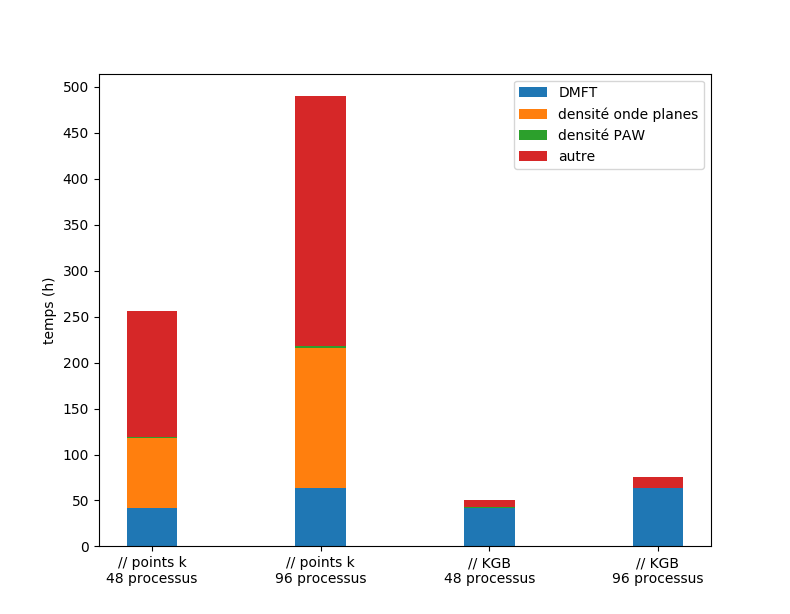
\includegraphics[width=0.7\textwidth]{pic/bargraph.png}
    \caption{Drastic effect of the use of paral\_kgb on a DMFT computation}
    \label{fig:bargraph.png}
  \end{figure}
\end{frame}


  {\nologo
    \begin{frame}[focus]
      Thank you for your attention !
    \end{frame}

    \begin{frame}[focus]
      Questions ?
    \end{frame}
  }

\end{document}
